\section{Results}
We have tested our implementation on a system comprising six slave nodes and one master
against a centralized system that made no RPCs. All nodes used for testing were
running Ubuntu 16.04.4 LTS on single-core \SI{2.6}{\giga\hertz} processors. In
addition, the nodes each had \SI{2}{\gibi\byte} of RAM and \SI{20}{\gibi\byte}
of disk space. The time taken by the distibuted system to process a set of
\(q\) range queries (\(0 \leq q \leq 1200\)) was found to be noticeably longer
than the time taken by the centralized system to process the same set of
queries. Figure~\ref{fig:graph-of-results} compares the execution time of the
distributed system with that of the centralized system. It was found that the
distributed system had an execution time of
\(\mathrm{t}_d(q) = 0.00452 q + 0.7 \mathrm{s}\)
with \(R^2 = 0.9919\) while the centralized system had an execution time of
\(\mathrm{t}_c(q) = 0.000152 q - 0.00231 \mathrm{s}\)
with \(R^2 = 0.9818\). Since the slope of \(\mathrm{t}_d(q)\) surpasses the
slope of \(\mathrm{t}_c(q)\), we expect the distributed system to perform more
slowly. This is an expected result due to the time required to perform RPCs and
execute the query planner. Despite the slower measured performance, using a
distributed system provides the benefits of fault tolerance and higher storage
capacity (in aggregate) as discussed in the Introduction. Further, while a
centralized system cannot be altered to provide fault tolerance, the execution
time of the distributed system could be improved through further optimization.
%
\begin{figure}
    \centering
    \includegraphics[width=\columnwidth]{results-graph}
    % 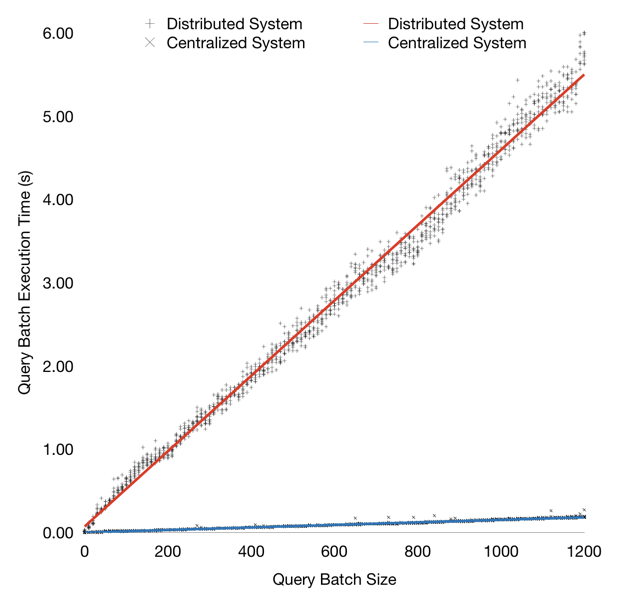
\includegraphics[width=\columnwidth]{query-experiment-results}
    \caption{Query Experiment Results}\label{fig:graph-of-results}
\end{figure}
